\documentclass[preprint,11pt,a4paper]{elsarticle}
\usepackage[a4paper,margin=2.5cm]{geometry}
\usepackage[utf8]{inputenc}
\usepackage[T1]{fontenc}
\usepackage{graphicx,amsmath,amssymb,array,booktabs,xurl,adjustbox,makecell,hyperref}
\renewcommand{\cellalign}{bl}\renewcommand{\theadalign}{bl}
\usepackage[switch]{lineno}
\usepackage{enumitem}
\setlist{nosep,leftmargin=*}
\hypersetup{hidelinks}
\DeclareUnicodeCharacter{2032}{\ensuremath{'}}
\DeclareUnicodeCharacter{2212}{\ensuremath{-}}
\DeclareUnicodeCharacter{03B1}{\ensuremath{\alpha}}
\DeclareUnicodeCharacter{03BA}{\ensuremath{\kappa}}
\DeclareUnicodeCharacter{00D7}{\ensuremath{\times}}
\DeclareUnicodeCharacter{2265}{\ensuremath{\geq}}
\DeclareUnicodeCharacter{2264}{\ensuremath{\leq}}
\DeclareUnicodeCharacter{2192}{\ensuremath{\rightarrow}}
\DeclareUnicodeCharacter{03C6}{\ensuremath{\phi}}
\DeclareUnicodeCharacter{00B1}{\ensuremath{\pm}}
\DeclareUnicodeCharacter{2248}{\ensuremath{\approx}}
\DeclareUnicodeCharacter{03C0}{\ensuremath{\pi}}
\DeclareUnicodeCharacter{03C4}{\ensuremath{\tau}}
\DeclareUnicodeCharacter{03C1}{\ensuremath{\rho}}
\DeclareUnicodeCharacter{0394}{\ensuremath{\Delta}}
\emergencystretch=3em
\renewcommand{\topfraction}{0.9}\renewcommand{\bottomfraction}{0.8}
\renewcommand{\textfraction}{0.07}\renewcommand{\floatpagefraction}{0.8}
\setcounter{topnumber}{3}\setcounter{bottomnumber}{2}\setcounter{totalnumber}{5}
\biboptions{numbers,sort&compress}
\AtBeginDocument{\setlength{\bibsep}{1pt plus 0.3pt}}
\journal{Mechanical Systems and Signal Processing}
\makeatletter
\let\ps@pprintTitle\ps@plain
\makeatother

\begin{document}
\begin{frontmatter}
\title{Phase-Dependent False-Alarm Calibration and Its Transport Across Engines in Full-Flight Aero-Engine Anomaly Detection}
\author[usyd]{Jinghang Mei\corref{cor1}}
\cortext[cor1]{Corresponding author. ORCID: \url{https://orcid.org/0009-0007-2901-3285}}
\ead{surnamemei05@gmail.com}
\address[usyd]{School of Electrical and Computer Engineering, The University of Sydney, Sydney, Australia}
\begin{abstract}
Residual-based anomaly detectors are usually given one alarm threshold calibrated to a nominal healthy false-alarm probability. Under nonstationary operation, such a pooled threshold controls only the exposure-weighted false-alarm rate. We audited this in full-flight aero-engine monitoring on the N-CMAPSS benchmark with residual principal component analysis (PCA), Isolation Forest and a past-only long short-term memory (LSTM) reconstruction network. Phase-dependent healthy false-positive rates, highest in descent, were discovered on the DS02 subset. A frozen protocol, applied once to held-out engines of the DS03 subset, reproduced the pre-specified pooled directional pattern (PCA: climb 0.877\%, cruise 0.912\%, descent 1.977\% at a 1\% target). Separately frozen post-confirmation analyses then examined calibration transport from two calibration engines to held-out audit engines. Retrospective phase-conditioned thresholds reduced pooled between-phase disparity and pooled maximum nominal calibration error in all 14 detector runs, although every paired bootstrap interval included zero. At matched healthy-flight false-flag rates, conditioning gave no general detection-delay advantage; earlier detection was confined mainly to low false-flag burdens. The pooled correction did not transport reliably to individual engines: two of the three short-flight audit engines, a flight class absent from calibration, became worse calibrated in every run, and weighting audit engines equally reversed the pooled improvement on DS02. A continuous operating-context quantile-regression threshold failed on different engines, and distance to calibration operating states did not explain the failures. Pooled phase-level correction therefore did not guarantee calibration transport across engines, and the strongest observed transport failures coincided with flight classes absent from calibration.
\end{abstract}
\begin{keyword}
condition monitoring \sep false-alarm calibration \sep nonstationary operating conditions \sep calibration transport \sep anomaly detection \sep aero-engine
\end{keyword}
\end{frontmatter}
\linenumbers

\section{Introduction}

\textbf{Detection as a calibrated threshold test.} Condition monitoring of machines and systems increasingly relies on data-driven detection statistics computed from residuals between measured signals and a model of nominal behaviour \cite{N1}. Whatever the model (principal-component reconstruction, an isolation-based score or a sequence reconstruction network), the monitoring decision is ultimately a threshold test: an alarm is raised when the statistic exceeds a level chosen for a nominal false-alarm probability. In aero-engine monitoring, false-alarm probability has long been an explicit design parameter of anomaly detection and alert-threshold placement \cite{ref2,ref11}. Frequent healthy alarms add review workload and can weaken the usefulness of a warning stream \cite{ref12}.

\textbf{Pooled thresholds under nonstationary operation.} The healthy distribution of a detection statistic is rarely stationary. Operating point, manoeuvres and ambient conditions change measured signals even when health is unchanged \cite{N2,N3,N4}. Schematically, a measured vector can be written as $x_t = f(h_t, o_t, d_t, \epsilon_t)$, where $h_t$ is health, $o_t$ the operating point, $d_t$ normal operating dynamics and $\epsilon_t$ measurement and model error. Operating-condition normalization removes part of the dependence on $o_t$ and $d_t$ before a statistic $s_t$ is formed and a decision $a_t = \mathbb{1}[s_t > \tau]$ is taken \cite{N2,N4,N5,N6}. When a single threshold $\tau$ is calibrated on pooled healthy data, it controls only the exposure-weighted false-alarm probability,

\[P(a=1\mid h) = \sum_{\phi} \pi_\phi \, P(a=1 \mid h,\phi),\]

where $\phi$ indexes operating contexts and $\pi_\phi$ is their share of healthy exposure. The pooled rate can meet its nominal target while individual contexts run well above or below it \cite{N7}. The expression for $x_t$ is conceptual, not an identified model.

\textbf{Context-specific thresholds are established.} The standard response is to condition the threshold on the operating context. Established examples, reviewed in Section 2, are:
\begin{itemize}
\item mode-specific control limits in multimode process monitoring \cite{N8};
\item constant-false-alarm-rate (CFAR) radar detectors \cite{N10};
\item category-conditional conformal calibration \cite{N7} and thresholds adapted to discrete environments under a false-alarm budget \cite{N45};
\item alarm thresholds set per operating condition, shaft-speed bin, flight condition or flight state in machinery, jet-engine and rotorcraft monitoring \cite{N22,N25,N26,N27};
\item time-variant and zone-specific alarm design for non-stationary process variables \cite{N39,N40}.
\end{itemize}

Conditioning a threshold on an operating category is therefore not new, and it is not proposed here.

\textbf{The open question is transport.} A context-specific threshold is calibrated on some units and then applied to others. Its guarantees rest on exchangeability between calibration and deployment data \cite{N20}, a particular calibration set can be unrepresentative \cite{N16}, and monitoring models may fail to transfer beyond the systems and conditions they were built on \cite{N21}. An improvement measured after pooling all audit data may therefore not hold for the individual engines on which alarms are raised. We call this property \emph{calibration transport}: whether a nominal healthy false-alarm calibration obtained on calibration engines remains valid, context by context, on other engines.

\textbf{The full-flight setting.} The N-CMAPSS benchmark simulates complete flights (climb, cruise and descent) driven by recorded flight conditions \cite{ref1}. Anomaly detection on N-CMAPSS has used increasingly sophisticated temporal and graph models, evaluated mainly through aggregate detection metrics \cite{ref7,ref8,ref9}. On simulated turbofan data, false-positive rates have been reported per operating mode, and a detector whose threshold was set on healthy cruise data alone flagged all data from the other modes \cite{N23}. Three questions are rarely made held-out endpoints:
\begin{itemize}
\item whether a pooled healthy calibration remains valid across normal flight phases;
\item whether a conditioned calibration that improves the pooled audit population also transports to individual engines;
\item what conditioning changes in abnormal-state detection when arms are compared at matched false-flag burden rather than at unequal operating points.
\end{itemize}

\textbf{Staged design.} The study proceeded in stages (Fig. 1):
\begin{figure}[htbp]
\centering
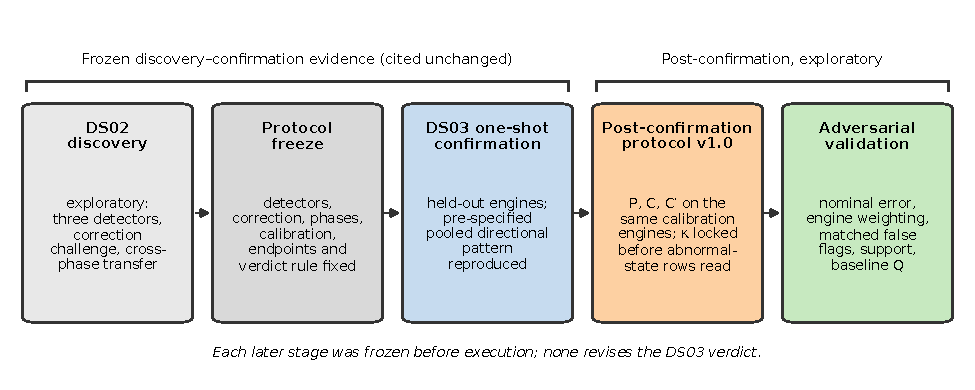
\includegraphics[width=\textwidth]{../figures/fig1_study_timeline.pdf}
\caption{Staged study design. DS02 discovery, the protocol freeze and the one-shot DS03 confirmation form the frozen evidence, which is cited unchanged. The post-confirmation protocol v1.0 (arms P, C and C′, with κ locked before abnormal-state rows were read once) and the adversarial validation (nominal error, engine weighting, matched false flags, operating support and the continuous baseline Q) were each frozen before execution. They are exploratory and do not revise the DS03 verdict.}
\label{fig:1}
\end{figure}
\begin{enumerate}
\item \textbf{DS02 discovery.} Three residual-based detectors, a correction challenge and a cross-phase threshold-transfer audit.
\item \textbf{Frozen DS03 confirmation.} All detector, correction, phase, calibration, endpoint and interpretation rules were frozen before a single evaluation on held-out engines.
\item \textbf{Post-confirmation transport analyses.} These were two further plans, each frozen before execution. A protocol comparing pooled with context-conditioned calibration was followed by an adversarial validation of it (nominal calibration error, engine weighting, matched false-flag delay, operating-support distance and a continuous contextual baseline).
\end{enumerate}

The frozen confirmation is reported unchanged; the post-confirmation analyses are exploratory and never qualify it.

\textbf{Research questions.}
\begin{itemize}
\item \textbf{RQ1 (frozen).} Under pooled calibration, do healthy row-level false-positive rates (FPRs) vary systematically across flight phases?
\item \textbf{RQ2 (frozen).} Do the tested static, derivative-based and finite-history operating-condition corrections sufficiently attenuate that dependence?
\item \textbf{RQ3 (frozen).} Does the pooled directional pattern reproduce across three detector implementations and on a frozen, held-out subset?
\item \textbf{RQ4 (post-confirmation).} Does context-conditioned calibration reduce nominal calibration error, not only between-phase disparity, and does a pooled improvement transport to individual engines?
\item \textbf{RQ5 (post-confirmation).} At matched healthy-flight false-flag rates, does conditioning change abnormal-state detection delay?
\item \textbf{RQ6 (post-confirmation).} Is the residual transport failure explained by the operating-state distance between audit and calibration data?
\end{itemize}

\textbf{Contributions.} The contribution is not phase-aware detection or regime-specific thresholding. It is a controlled audit of nominal healthy-FPR calibration and its transport under full-flight operation:
\begin{enumerate}
\item \textbf{Pooled calibration and cross-phase transfer.} Under pooled calibration, healthy FPR depended on flight phase for three residual-based detectors, and phase-specific thresholds transferred unevenly between phases.
\item \textbf{Discovery separated from confirmation.} The DS02 pattern was reproduced by a frozen one-shot DS03 evaluation, with engine- and seed-level exceptions reported.
\item \textbf{A post-confirmation transport audit.} Retrospective phase-conditioned thresholds removed most of the pooled phase-composition error, but the correction did not transport reliably to engines. The negative results are retained: no general delay advantage at matched false-flag rates, a continuous contextual baseline that failed on other engines, and support distance that did not explain the failures.
\item \textbf{An evaluation protocol for monitoring studies.} Nominal calibration error, between-context disparity, engine-weighted summaries and matched false-flag delay are reported together, under frozen plans with exact reproduction gates and re-derivable numbers.
\end{enumerate}

\textbf{Scope.} The work provides calibration evidence for simulated N-CMAPSS subsets. It does not propose a detector or a threshold policy, identify a mechanism, or validate deployment on aircraft. The calibration question is not specific to aero-engines. It arises wherever one detection threshold, or one set of context-specific thresholds, is calibrated on part of a fleet and applied to other units operating under changing conditions, for example wind turbines \cite{N1,N4}, gearboxes \cite{N3}, gas turbines \cite{N13} and civil structures subject to environmental and operational variability \cite{N2,N5,N6}.

\section{Related work}

\subsection{Operating-condition variability in machinery health monitoring}

Environmental and operational variability is a central problem in structural and machine monitoring, because changing conditions alter measured features and can mask or mimic damage \cite{N2}. Established responses include:
\begin{itemize}
\item data normalization and factor analysis before control charting \cite{N2,N5};
\item models of the healthy response driven by measured operating parameters \cite{N4};
\item regime-switching response surfaces for structures whose behaviour changes abruptly between regimes \cite{N6};
\item machine-condition methods that first infer the operating condition and then assess condition relative to it, for gearboxes under fluctuating operation \cite{N3}.
\end{itemize}

For gas-turbine engines, classical practice monitored a restricted set of operating points or corrected measurements to reference conditions \cite{N35}. Flight-condition-aware monitoring predates full-flight benchmarks. It includes flight-stage normalization of health and usage indicators \cite{ref4}, models of flight-data interrelations within a specified flight regime \cite{ref3}, and fleet monitoring with adaptive performance models across variable conditions \cite{ref5}.

N-CMAPSS replaced the snapshot-oriented C-MAPSS benchmark with complete simulated flights and assigns each engine a flight class \cite{ref1}; its flight phases differ between flight classes, which motivates phase-wise alignment when models are transferred between flight-class sub-fleets \cite{N28}. Operating-condition normalization and regime-specific modelling are therefore not contributions of this paper.

\subsection{Condition-aware anomaly detection and adaptive alarm thresholds}

\textbf{Anomaly detection under changing conditions.} For gas turbines under frequently changing operating conditions, anomaly detectors have been trained on a single condition and evaluated by aggregate discrimination (AUROC), with conventional vibration limits described as hard limits that do not adjust to conditions \cite{N13}. A variational autoencoder conditioned on operating-condition variables has been used to decouple equipment state from operating conditions in power-plant gas turbines, and it was evaluated against six detection methods \cite{N38}. On N-CMAPSS, residual models have been used to study training-data contamination \cite{ref7}, information-based fault detection has been evaluated \cite{ref8}, and a physics-guided spatiotemporal graph model has been assessed through ROC-AUC and F1 \cite{ref9}. Residual-based detectors with thresholds set on healthy data have been compared by unit-level false positives and detection delay using cruise data only, because cruise is more stable than take-off or landing \cite{N42}. For an aviation piston engine, detection metrics reported per power-lever phase under one global threshold were worst in climb, with phase-adaptive thresholds and cross-engine transfer left for future work \cite{N43}. These studies make detection performance, not the phase-conditional validity of a healthy calibration, the endpoint.

\textbf{Adaptive and automatic thresholds.} Adaptive thresholds for aero-engine fault detection have been set over flight-envelope subareas \cite{ref6}. Automatic, data-driven threshold setting for vibration-based anomaly detection is an active topic in this journal \cite{N14}. In machine-sound anomaly detection, optimal decision thresholds differ across operating domains, so a single threshold across domains degrades performance \cite{N37}.

\textbf{Condition-specific alarm thresholds.} The closest precedents are condition-specific thresholds motivated by false alarms:
\begin{itemize}
\item \textbf{Multimode process monitoring.} Zhao et al. noted that a single-region model ``would always trigger continuous warnings'' in other normal modes. Mode-specific principal-component control limits reduced such false alarms \cite{N8}. Mode-specific control limits for PCA residuals therefore predate this work.
\item \textbf{Machinery alarms.} Toshkova et al. set extreme-value alarm thresholds per identified operating condition and reported a more reliable health indication than with uniform thresholds \cite{N22}.
\item \textbf{Aero-engines and rotorcraft.} Clifton et al. set novelty thresholds per shaft-speed bin for jet-engine vibration \cite{N27}. Wang et al. segmented aero-engine monitoring by flight condition \cite{N25}. Lee et al. optimized thresholds per flight state for rotorcraft health and usage monitoring, where condition-agnostic thresholds caused frequent false alarms \cite{N26}.
\item \textbf{Alarm-system design.} Alarm design balances false-alarm rate, missed-alarm rate and alarm delay \cite{N32}. Asaadi et al. assessed univariate alarm systems for a process variable affected by an intermittent fault, modelled as a time-variant finite mixture, through the false-alarm rate, missed-alarm rate and averaged alarm delay over time \cite{N39}. Their operational zone-specific design segments a process variable by change-point detection into normal, rising, fault and return-to-normal zones and evaluates zone-wise indices \cite{N40}. These zones are stages of fault evolution in one variable, not normal operating contexts, and neither study evaluates whether an alarm calibration transports across units.
\end{itemize}

\textbf{Per-mode false-positive rates.} Michau and Fink reported false-positive rates for five operating modes of simulated turbofan data (take-off, cruise at two altitudes, descent and landing). A detector whose threshold was set on healthy cruise data alone flagged all data from the other modes \cite{N23}. This is the closest demonstration that a calibration obtained in one context does not carry to another. It concerns transfer between operating modes rather than the validity of a pooled or context-conditioned calibration across engines.

\subsection{Calibration validity, threshold transfer and the remaining gap}

\textbf{Calibration validity.} Distribution-free calibration clarifies what a pooled threshold guarantees:
\begin{itemize}
\item Conformal p-values computed against a held-out inlier calibration set control the false-positive rate on average over calibration sets. A particular calibration set can be ``unlucky'' \cite{N16}.
\item Validity within categories requires category-conditional calibration \cite{N7}; monitoring thresholds can likewise be adapted to discrete environments while a false-alarm budget is distributed over an a priori partition \cite{N45}.
\item Conformal threshold setting has been compared with classical thresholds for PCA and autoencoder fault detectors as a way to control false alarms \cite{N41}.
\item In heterogeneous fleets, fleet-level normal models can be inefficient at individual units, which has motivated calibrating each unit against a similar sub-fleet with a bounded false-alarm probability \cite{N44}.
\item All of these guarantees rest on exchangeability between calibration and deployment data, which drift violates \cite{N20}. Under covariate shift, validity requires likelihood-ratio weighting \cite{N30}.
\end{itemize}

\textbf{Changing nuisance statistics.} Signal-processing detection faces the same issue. Subspace damage-detection tests fail when the excitation statistics change between the reference and monitored states \cite{N15}. CFAR processors keep a constant false-alarm rate only by adapting to local clutter, and their behaviour at clutter edges is a separate design concern \cite{N10}.

\textbf{Delay and false-alarm burden.} Detection delay must be tied to the false-alarm rate. Sequential change detection defines and optimizes delay for a fixed mean time between false alarms \cite{N17}, and the ProDiMES benchmark fixed a common flight-level false-alarm target before comparing aircraft-engine gas-path detection rates and latency \cite{N24}.

\textbf{The remaining gap.} In a documented search we did not find a study that combines:
\begin{itemize}
\item an audit showing that a pooled nominal threshold on full-flight engine residuals controls only the exposure-weighted healthy FPR while climb, cruise and descent FPRs differ;
\item cross-phase threshold transfer as a pre-specified endpoint, with every phase present in calibration;
\item a frozen discovery-to-confirmation separation for that question;
\item a post-confirmation evaluation of whether an apparent pooled phase-level correction transports to individual engines, with nominal calibration error, engine weighting, matched false-flag delay, a continuous contextual baseline and operating-support distance.
\end{itemize}

No priority is claimed for context-aware monitoring, regime-specific thresholds or adaptive thresholding. The contribution is the controlled calibration-transport audit.

\section{Methodology}

The analysis chain is $x_t \rightarrow r_t \rightarrow s_t \rightarrow a_t$: a sensor vector $x_t$, an operating-condition residual $r_t$, a detector score $s_t$ and a row alarm $a_t = \mathbb{1}[s_t > \tau(\cdot)]$. A pooled threshold $\tau$ is a single calibration quantile. A conditioned threshold $\tau_c$ is computed within a context $c$ (a retrospective phase, a past-only regime, or a continuous operating state). A pooled quantile sets $\sum_\phi \pi_\phi P(a=1\mid h,\phi)$ to the nominal level, whereas a conditioned quantile targets each $P(a=1\mid h,\phi)$ on the calibration engines. Transport is the question of whether either target, set on calibration engines, holds on audit engines, both pooled over them and engine by engine.

\subsection{Dataset and staged study design}

N-CMAPSS provides simulated run-to-failure trajectories of turbofan engines flown along recorded flight profiles \cite{ref1}. Each engine flies one flight class: class 1 comprises short flights (1–3 h) at low altitude and speed, class 2 flights of 3–5 h, and class 3 the longest and highest flights (5–7 h) \cite{ref1}. The analysis used subset DS02 for exploratory discovery and subset DS03 for frozen confirmation (Table 1). The study was staged as follows (Fig. 1).
\begin{table}[htbp]
\centering
\small
\caption{Datasets, engine partitions with flight classes, phase roles and calibration arms.}
\label{tab:1}
% Datasets, partitions, phase and calibration roles
\begin{tabular}{>{\raggedright\arraybackslash}p{0.25\textwidth}>{\raggedright\arraybackslash}p{0.31\textwidth}>{\raggedright\arraybackslash}p{0.36\textwidth}}
\toprule
Item & DS02 & DS03 \\
\midrule
Role & exploratory discovery & frozen one-shot confirmation (held-out official-test engines) \\
\midrule
Post-confirmation role & reused for exploratory transport analyses & reused for exploratory transport analyses \\
\midrule
Model-fitting engines (flight class) & 2 (3), 5 (3), 10 (3), 16 (3) & 1 (1), 2 (2), 3 (2), 5 (1), 6 (3), 7 (2), 9 (1) \\
\midrule
Calibration engines (flight class) & 18 (3), 20 (3) & 4 (2), 8 (3) \\
\midrule
Audit engines (flight class) & 11 (3), 14 (1), 15 (2) & 10 (3), 11 (3), 12 (1), 13 (3), 14 (1), 15 (2) \\
\midrule
Audit engines of a class absent from calibration & 14 (class 1), 15 (class 2) & 12 (class 1), 14 (class 1) \\
\midrule
Healthy calibration / audit flights & 32 / 76 & 40 / 148 \\
\midrule
Abnormal-state (hs = 0) rows read, once & 820,630 & 2,956,881 \\
\midrule
Phase labels & retrospective climb/cruise/descent (P, C); past-only regimes (C$'$) & retrospective climb/cruise/descent (P, C); past-only regimes (C$'$) \\
\midrule
Calibration arms compared & P, C, C$'$; Q (healthy side only) & P, C, C$'$; Q (healthy side only) \\
\bottomrule
\end{tabular}

\end{table}

\textbf{Discovery and freeze.} Detector families, the correction specification, the calibration rule, the phase definition, the evaluation endpoints and the interpretation rule were fixed before the DS03 audit outcomes were examined. DS03 was evaluated once under the frozen primary protocol. DS02 estimates were not treated as confirmation.

\textbf{Post-confirmation analyses.} After the confirmation, DS02 and DS03 were reused for exploratory transport analyses under two further plans, each committed before execution:
\begin{itemize}
\item \textbf{Protocol v1.0.} This protocol compared calibration arms and locked all calibration-derived quantities before any abnormal-state row was read. Abnormal-state rows were then read once per dataset (820,630 DS02 and 2,956,881 DS03 rows).
\item \textbf{Adversarial validation plan.} This plan added calibration-quality, engine-weighting, matched-delay, support and baseline analyses. It reread no abnormal-state row.
\end{itemize}

Every stage began with exact reproduction gates (rescored healthy vectors equal to the frozen fingerprints bit for bit; recomputed tables, locks and bootstrap summaries equal to the committed ones), and a 186-file hash manifest of the frozen evidence was verified before and after every run. DS03 is described as held out only for the frozen confirmation.

\subsection{Engine-disjoint fitting, calibration and audit partitions}

The engine was the partitioning and top-level inferential unit, and timestamped observations were nested within flights identified by engine and cycle. Model-fitting, calibration and audit engines were disjoint (Table 1). LSTM epoch selection, model fitting and calibration followed this frozen allocation, and no detector, correction or threshold setting was changed after audit outcomes were available.

Flight class is a descriptive engine attribute that was never used to change a rule. In DS02 every model-fitting and calibration engine is class 3, so audit engines 14 (class 1) and 15 (class 2) come from classes absent from calibration. In DS03, calibration covers classes 2 and 3 (engines 4 and 8), so class-1 audit engines 12 and 14 are the absent-class engines; class 1 does appear among the DS03 model-fitting engines.

\subsection{Healthy and abnormal-state labels}

The detectors used 14 measured sensor channels. Four operating descriptors (altitude, Mach number, throttle-resolver angle and fan-inlet temperature; together $W$) were used for residualization and for the contextual analyses. The N-CMAPSS health-state annotation was never a detector input. It has two roles:
\begin{itemize}
\item It selects healthy ($hs = 1$) rows for fitting, threshold calibration and healthy false-alarm evaluation.
\item In the post-confirmation analyses, it defines abnormal-state ($hs = 0$) rows and the labelled onset, the first flight with $hs = 0$, from which detection delay is counted in flights.
\end{itemize}

Because $hs = 0$ marks the simulated onset of degraded operation rather than a discrete fault event, abnormal-state endpoints are reported as alarm rates and delays relative to that labelled onset.

\subsection{Retrospective phase definition}

\textbf{Primary rule.} For each complete flight, the cruise interval ran from the first through the last sample whose altitude reached at least 90\% of the flight's observed altitude range above its minimum. Earlier samples were labelled climb and later samples descent. These labels require the complete flight; they serve retrospective stratification only and are not available during a flight.

\textbf{Alternative retrospective rule (DS02 sensitivity only).} Cruise was defined by 85\% of the altitude range together with an absolute centred 60-s altitude rate of at most 2 ft/s (0.61 m/s).

\textbf{Past-only regimes.} For the past-only regime-conditioned arm, each row was labelled ascending, level or descending from its trailing 60-s altitude rate, with a dead-band of ±2.0 ft/s (0.61 m/s; altitude sampled at 1 Hz, with shorter trailing windows at the start of each flight). Only current and past samples of the same flight are used. This rule reuses the window and limit of the alternative rule, but it is trailing and has no altitude-fraction condition.

\subsection{Operating-condition residualization}

The exploratory DS02 correction comparison considered three bases: static operating state, static plus first differences, and finite history. All confirmation and post-confirmation detector analyses used the finite-history specification. For each flight, its descriptors were:
\begin{itemize}
\item the current operating state and its first differences;
\item trailing means, standard deviations and endpoint slopes over 30- and 120-sample windows (30 and 120 s at 1 Hz).
\end{itemize}

Descriptor construction reset at flight boundaries and used no future samples. A ridge regression (penalty 1.0) predicted the measured sensors from these descriptors. Its basis had cubic terms of the instantaneous operating state, linear and squared dynamic terms, and interactions between the instantaneous state and its first differences. Regression fitting and residual standardization used model-fitting engines only.

\subsection{PCA, Isolation Forest and past-only LSTM scores}

\textbf{Residual PCA.} Five components were fitted to the standardized residuals. The row score was the mean squared reconstruction error.

\textbf{Isolation Forest.} The forest used 200 trees, a maximum sample size of 8192 and automatic contamination, with seeds 0, 1 and 2. The score was the negative of the library \texttt{score\_samples} output.

\textbf{Past-only LSTM.} A sequence-reconstruction network whose forward recurrences use only the current and preceding samples within a window:
\begin{itemize}
\item \textbf{Architecture.} Two 16-unit forward LSTM layers around an eight-feature per-time-step bottleneck, applied to 256-row windows within each flight, with a per-row mean squared reconstruction error.
\item \textbf{Fitting.} Adam with learning rate 0.001 and batch size 256, and engine-disjoint epoch selection with at most 600 epochs and patience 6, for seeds 0, 1 and 2.
\item \textbf{Convergence.} The DS02 seed-0 selection reached the epoch ceiling while validation loss was still improving. It is retained as a convergence limitation without test-informed retuning (Supplementary Figs. S1–S2).
\end{itemize}

The seven detector runs per dataset (one PCA run and three seeds each for Isolation Forest and the LSTM) are the units over which post-confirmation results are counted.

\subsection{Pooled calibration and cross-phase transfer}

\textbf{Pooled calibration (P).} For each detector run, pooled healthy calibration scores set nominal row-level FPR targets α of 0.5\%, 1\% and 2\% by the empirical upper quantile (``higher'' order statistic); 1\% was primary. Phase-specific healthy FPRs were computed as alarmed healthy rows over healthy rows, pooled over audit engines and per engine.

\textbf{Frozen endpoints.} The directional contrasts were descent minus climb and descent minus cruise. For cross-phase transfer, a threshold calibrated within one phase was applied to each of the other phases. The frozen flight-level burden endpoint was ``healthy flights with any alarm''. It is kept separate throughout from the κ-based false-flag rate of Section 3.9.4.

\textbf{Uncertainty.} Two thousand hierarchical bootstrap replicates resampled calibration and audit data separately (engines, then flights within engines) and re-estimated thresholds in every replicate. No timestamp-level test was used. Intervals pertain to individual detector runs; no interval for a seed mean was computed, and interval endpoints were never averaged.

\subsection{Frozen DS03 confirmation}

The frozen protocol specified the primary phase rule, the history correction, the three detector families, pooled calibration at the three targets, the directional contrasts and the verdict rule before the DS03 audit engines were scored. The confirmation asked whether the pooled directional pattern (descent above climb and cruise under pooled calibration) reproduced. Per-engine directional exceptions and individual-run intervals were reported alongside the verdict. The confirmation was run once and is not revised by any later analysis.

\subsection{Post-confirmation calibration-transport analyses}

All post-confirmation analyses reuse the frozen detectors, scores and engine partitions; calibration-derived quantities use healthy calibration engines only, and nothing was changed after outcomes were seen.

\subsubsection{Phase-conditioned thresholds}

The arms share the same healthy calibration rows:
\begin{itemize}
\item \textbf{P:} the frozen pooled thresholds;
\item \textbf{C, retrospective phase-conditioned calibration:} per-phase upper quantiles, which are the diagonal of the frozen transfer design and were therefore observed before these analyses;
\item \textbf{C′, past-only regime-conditioned calibration:} per-regime upper quantiles, with regimes from the trailing altitude rate (Section 3.4).
\end{itemize}

C requires complete-flight labels and is a retrospective diagnostic. C′ uses current and past samples only and is examined as an implementable alternative, not as a deployed system.

\subsubsection{Continuous contextual calibration baseline}

Coarse phase labels might cause any transport failure of C. To test that objection, a continuous contextual threshold (Q) was added as an adversarial control, not as a proposed method. Its specification was fixed before execution:
\begin{itemize}
\item \textbf{Model.} Linear quantile regression of the detector score at level $1-\alpha$ on a quadratic response surface of the four standardized operating descriptors $W$: four linear terms, four squares and six pairwise products (14 terms plus an intercept).
\item \textbf{Fitting.} The model was solved exactly by linear programming (unpenalized, HiGHS solver) on every fifth healthy calibration row, per detector run and target, with no tuning and no phase input.
\item \textbf{Alarm rule.} A row alarms when its score exceeds the predicted quantile. The flight-level κ is computed from healthy calibration flights, as for the other arms.
\end{itemize}

Q was pre-specified to run only if C reduced between-phase disparity in at least 5 of 7 runs per dataset, which held. Only its healthy-side endpoints were evaluated, because its abnormal-state endpoints would have required a new read of abnormal-state rows.

\subsubsection{Calibration-quality metrics}

For each arm and target, with phase FPRs $\{\mathrm{FPR}_\phi\}$ over climb, cruise and descent:
\begin{itemize}
\item \textbf{A1, between-phase disparity:} $\max_\phi \mathrm{FPR}_\phi - \min_\phi \mathrm{FPR}_\phi$;
\item \textbf{A2, maximum nominal calibration error:} $\max_\phi |\mathrm{FPR}_\phi - \alpha|$;
\item \textbf{A3, root-mean-square nominal calibration error:} computed over the three phases;
\item \textbf{A5, overall-FPR error:} $|\mathrm{FPR} - \alpha|$ over all healthy audit rows.
\end{itemize}

Disparity measures only equality between phases, whereas nominal calibration error measures distance from α. A disparity reduction is called a calibration improvement only when the nominal-error metrics also decrease.

\textbf{Weightings.} Every metric was computed row-pooled over audit engines (the frozen estimand), with audit engines weighted equally, and per engine.

\textbf{Categories.} Each comparison with P (dataset × run × target × arm) fell into one of four pre-specified categories:
\begin{enumerate}
\item disparity and nominal calibration both improve;
\item disparity improves but nominal calibration does not;
\item mixed;
\item conditioning worsens both.
\end{enumerate}

\textbf{Wording rule.} The pre-specified rule allowed the wording ``improved nominal phase-wise calibration'' only for category 1 in at least 6 of 7 runs at 1\%, at least 5 of 7 at the other targets, and no contradiction in a majority of engines.

\textbf{Uncertainty.} Paired arm-minus-P intervals extended the frozen bootstrap resampling plans (engines, then flights; thresholds re-estimated; 2000 replicates). Each claim was also classified across the three targets as invariant, mostly invariant, target-sensitive or reversed.

\subsubsection{Matched false-flag delay analysis}

\textbf{Flight rule.} A flight's alarm fraction $r(f)$ is its share of alarmed rows, and the flight is flagged if $r(f) > \kappa$. For each run, arm and target, κ was locked in advance at the 0.95 ``higher'' quantile of healthy calibration-flight alarm fractions, a nominal 5\% healthy-flight false-flag rate. It is the second-largest of 32 (DS02) or 40 (DS03) calibration flights.

\textbf{Delay and burden.} The realized healthy-flight false-flag rate (FFR) is the share of healthy audit flights that are flagged. An audit engine's detection delay is the number of flights from the labelled onset to its first flagged post-onset flight; it is censored if no post-onset flight is flagged. Delays are summarized by the lower median over audit engines, with censored engines ranked last.

\textbf{Matching.} Comparing arms at their own locked κ confounds delay with false-flag burden, because each locked κ yields a different realized FFR. Arms were therefore compared at matched realized FFR:
\begin{itemize}
\item \textbf{Operating characteristic.} κ was swept over a calibration-only grid: zero, the healthy calibration-flight alarm fractions, and 400 fixed log-spaced values in $[10^{-4}, 1]$. No audit or abnormal-state quantity entered the grid.
\item \textbf{Anchors.} At each anchor FFR (2.5\%, 5\%, 10\%, 15\% and 20\%), each arm used the grid point with the nearest realized FFR.
\item \textbf{Support.} A match was supported only within one healthy-flight step of the anchor ($1/N_h$, with $N_h$ = 76 in DS02 and 148 in DS03). Delays were never interpolated or extrapolated.
\end{itemize}

\textbf{Labels.} At each supported anchor, the per-engine arm-minus-P delay differences were summarized by their lower median. A run was labelled:
\begin{itemize}
\item ``earlier at matched burden'' if the difference was negative at a majority of its supported anchors and positive at none;
\item ``later'' in the mirror case;
\item ``equal'' if it was zero at every supported anchor;
\item ``mixed'' otherwise.
\end{itemize}

The statement ``improves detection delay'' required the earlier label in at least 5 of 7 runs, together with a lower curve-level mean than P.

\textbf{Curve-level mean.} It is the mean of the matched median delay over a grid of realized FFR from 2.5\% to 20\% in 0.25-point steps (71 points), using at each grid point the nearest operating point within one healthy-flight step and excluding grid points without one. It is therefore a normalized partial area under the median-delay operating characteristic over a range of false-flag rates that every arm covers, with no interpolation.

\subsubsection{Engine weighting and transport analysis}

\textbf{Transport metrics.} Transport was assessed through:
\begin{itemize}
\item per-engine metrics;
\item the equal-engine summaries;
\item the sign agreement between row-pooled and equal-engine paired differences.
\end{itemize}

A post-plan descriptive decomposition (Supplement) splits the equal-cell mean squared nominal error over engine × phase cells into overall bias, phase, engine and interaction components.

\textbf{C0, phase effect without support mismatch.} Pooled thresholds were applied to the calibration engines themselves, both in-sample and from one calibration engine to the other. Calibration-to-audit mismatch is absent there by construction.

\textbf{Operating-support distance.} With operating descriptors standardized by calibration statistics, each healthy audit row's support distance was its Euclidean distance to the nearest healthy calibration row of the same retrospective phase. Secondary versions ignored phase or added the 120-s trailing slopes, and the distance between the two calibration engines served as the reference scale. Spearman correlations between median cell distance and $|\mathrm{FPR} - \alpha|$ under C were computed across engine × phase cells, per run, with leave-one-engine-out ranges; rows were never treated as independent units. A pre-specified rule classified the association as supported, not supported, or indeterminate because of the small engine count.

\subsection{Implementation, reproducibility and use of AI tools}

The pipeline was implemented in Python 3.12 (NumPy, pandas, scikit-learn and PyTorch; package versions are locked in the repository), and every stage writes run records with the hashes of its inputs and analysis module. Generative AI coding assistants were used in the research process under the author's direction:
\begin{itemize}
\item \textbf{OpenAI ChatGPT and Codex (OpenAI)} supported code development and debugging for the discovery and confirmation pipeline.
\item \textbf{Claude (Anthropic; Claude Opus 5.5, used through the Claude Code tool)} wrote the post-confirmation and adversarial-validation code, ran those analyses in the author's environment under the frozen plans, and wrote the figure, table and verification scripts.
\end{itemize}

The author set the research questions, approved every protocol and plan before execution, and reviewed the code and outputs. Correctness rests on the exact reproduction gates (Section 3.1), automated tests, and scripts that re-derive every reported number; the pipeline has not been independently reimplemented. The figures are data plots and a schematic drawn by these scripts, and no generative image tool was used.

\section{Results}

Sections 4.1–4.7 report the frozen discovery and confirmation results unchanged. Section 4.8 is post-confirmation and exploratory.

\subsection{DS02 discovery}

At the primary nominal 1\% pooled calibration target, PCA healthy row-level FPR was 0.125\% in climb, 0.428\% in cruise and 3.459\% in descent (Fig. 2, Table 2). The descent-minus-climb and descent-minus-cruise contrasts were +3.335 and +3.031 percentage points (pp).
\begin{figure}[htbp]
\centering
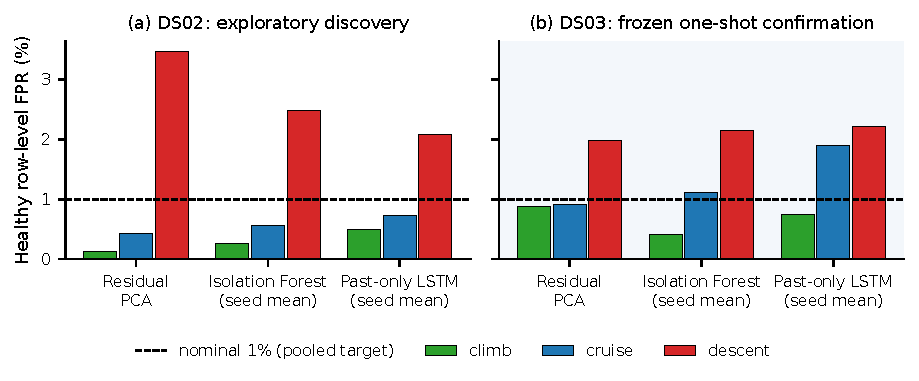
\includegraphics[width=\textwidth]{../figures/fig2_frozen_pooled_phase_fpr.pdf}
\caption{Frozen pooled-threshold healthy row-level FPR by flight phase at the 1\% target: (a) DS02 exploratory discovery; (b) DS03 frozen one-shot confirmation on held-out engines. Isolation Forest and LSTM bars are frozen seed means. The dashed line marks the nominal 1\% pooled target, which constrains the pooled rate, not each phase. Evidence IDs are listed in Table 2.}
\label{fig:2}
\end{figure}
\begin{table}[htbp]
\centering
\small
\caption{Frozen pooled-calibration audit at the 1\% target: phase FPRs, contrasts and worst cross-phase transfer FPR, with evidence IDs. Isolation Forest and LSTM rows are frozen seed means.}
\label{tab:2}
\begin{adjustbox}{max width=\textwidth}
% Frozen pooled-calibration audit at the 1% target
\begin{tabular}{llllllllll}
\toprule
Dataset & Detector & Climb & Cruise & Descent & Overall & \makecell{Descent\\$-$ climb} & \makecell{Descent\\$-$ cruise} & \makecell{Worst\\transfer FPR} & \makecell{Evidence\\IDs} \\
\midrule
DS02 (discovery) & Residual PCA & 0.125\% & 0.428\% & 3.459\% & 1.363\% & +3.335 pp & +3.031 pp & 15.555\% & \makecell{E000106--\\E000113} \\
 & \makecell{Isolation Forest\\(seed mean)} & 0.268\% & 0.558\% & 2.487\% & 1.127\% & +2.219 pp & +1.928 pp & 27.281\% & \makecell{E002626--\\E002633} \\
 & \makecell{Past-only LSTM\\(seed mean)} & 0.488\% & 0.729\% & 2.080\% & 1.118\% & +1.592 pp & +1.351 pp & 5.954\% & \makecell{E002986--\\E002993} \\
\midrule
DS03 (confirmation) & Residual PCA & 0.877\% & 0.912\% & 1.977\% & 1.341\% & +1.100 pp & +1.066 pp & 6.716\% & \makecell{E010946--\\E010952} \\
 & \makecell{Isolation Forest\\(seed mean)} & 0.409\% & 1.104\% & 2.142\% & 1.355\% & +1.733 pp & +1.038 pp & 9.386\% & \makecell{E012857--\\E012863} \\
 & \makecell{Past-only LSTM\\(seed mean)} & 0.751\% & 1.889\% & 2.215\% & 1.736\% & +1.464 pp & +0.325 pp & 5.308\% & \makecell{E013130--\\E013136} \\
\bottomrule
\end{tabular}

\end{adjustbox}
\end{table}

The corresponding Isolation Forest seed-mean FPRs were 0.268\%, 0.558\% and 2.487\% (contrasts +2.219 and +1.928 pp). For the LSTM, the seed-mean FPRs were 0.488\%, 0.729\% and 2.080\% (contrasts +1.592 and +1.351 pp). Under pooled calibration, descent therefore had the highest healthy FPR across the three tested implementations. The nominal 1\% target applied to pooled healthy calibration scores; it did not constrain each audit phase to 1\% FPR.

\subsection{Correction sensitivity}

For DS02 PCA, the descent-minus-climb contrasts were +2.854, +3.045 and +3.335 pp under static, static-plus-derivative and finite-history correction, respectively. The descent-minus-cruise contrasts were +2.418, +2.648 and +3.031 pp. The tested corrections therefore did not sufficiently attenuate the dependence: both contrasts remained positive under every tested correction and did not shrink. This exploratory comparison was not repeated on DS03 (Supplementary Table S2).

\subsection{Cross-detector consistency}

With the common history correction and pooled calibration, DS02 overall healthy row-level FPRs were 1.363\% for PCA, 1.127\% for the Isolation Forest seed mean and 1.118\% for the LSTM seed mean. The descent elevation was observed across the three tested implementations. They share preprocessing and calibration, so this does not establish detector independence.

\subsection{Cross-phase threshold transfer}

On DS02, the worst off-diagonal healthy row-level FPR after phase-specific calibration was 15.555\% for PCA. The arithmetic means of the per-seed maxima were 27.281\% for Isolation Forest and 5.954\% for the LSTM. The corresponding DS03 values were 6.716\%, 9.386\% and 5.308\%. In every run on both subsets, the maximum cell applied a climb-calibrated threshold to healthy descent rows (Supplementary Table S6). Off-diagonal cells are cross-phase transfer FPRs, and diagonal cells are within-phase healthy FPRs. Neither is a pooled-threshold phase FPR. The diagonal is the phase-conditioned arm examined in Section 4.8.

\subsection{Cluster-aware uncertainty and engine heterogeneity}

The audit sets contain three DS02 and six DS03 engines, so reversals in individual engines matter.
\begin{itemize}
\item \textbf{DS02 PCA.} The hierarchical-bootstrap 95\% intervals were [+2.070, +5.629] pp for descent minus climb and [+1.808, +5.261] pp for descent minus cruise.
\item \textbf{DS02 LSTM.} The descent-minus-climb intervals for seeds 1 and 2 included zero: [−0.022, +2.817] and [−0.347, +2.802] pp.
\item \textbf{DS03 PCA.} The intervals were [+0.434, +1.785] and [+0.560, +1.573] pp.
\item \textbf{DS03 LSTM.} Every descent-minus-cruise interval included zero.
\end{itemize}

Per-engine values are given in Supplementary Tables S4–S5.

\subsection{Frozen DS03 confirmation}

At the pre-specified primary target, the pooled climb, cruise and descent FPRs were:
\begin{itemize}
\item PCA: 0.877\%, 0.912\% and 1.977\%;
\item Isolation Forest seed means: 0.409\%, 1.104\% and 2.142\%;
\item LSTM seed means: 0.751\%, 1.889\% and 2.215\%.
\end{itemize}

The pooled descent-minus-climb and descent-minus-cruise contrasts were:
\begin{itemize}
\item PCA: +1.100 and +1.066 pp;
\item Isolation Forest seed mean: +1.733 and +1.038 pp;
\item LSTM seed mean: +1.464 and +0.325 pp.
\end{itemize}

The pre-specified pooled directional pattern was therefore reproduced (Fig. 2, Table 2). Three of 42 per-engine detector/seed rows were directional exceptions, all for LSTM seed 2. All three individual-seed LSTM descent-minus-cruise intervals included zero: [−0.222, +1.201], [−0.270, +1.158] and [−0.582, +1.025] pp. The pooled pattern therefore reproduced without uniform engine-level replication.

\subsection{Phase-rule sensitivity}

Under the alternative retrospective rule (85\% of the altitude range and an absolute centred 60-s altitude rate of at most 2), the pooled descent-minus-climb and descent-minus-cruise contrasts remained positive on DS02:
\begin{itemize}
\item PCA: +3.432/+3.293 pp;
\item Isolation Forest: +2.383/+2.256 pp;
\item LSTM: +1.803/+1.756 pp.
\end{itemize}

The frozen DS03 confirmation used the primary rule only (Supplementary Table S3).

\subsection{Post-confirmation calibration transport}

All results in this section are exploratory point-estimate patterns over the seven detector runs per dataset, reported with paired bootstrap intervals and engine-level results (Tables 3–5; every run, engine, target and interval is in the Supplement).
\begin{table}[htbp]
\centering
\small
\caption{Post-confirmation calibration quality at the 1\% target (percentage points; range over the seven detector runs): between-phase disparity A1, maximum and RMS nominal error A2 and A3, overall-FPR error A5, the number of runs in which each arm is below P, and the equal-engine A2. All paired intervals include zero.}
\label{tab:3}
\begin{adjustbox}{max width=\textwidth}
% Post-confirmation calibration quality at the 1% target
\begin{tabular}{llllllll}
\toprule
Dataset & Arm & \makecell{A1\\disparity} & \makecell{A2 max\\error} & \makecell{A3 RMS\\error} & \makecell{A5 overall\\error} & \makecell{Runs below P\\(A1/A2/A3/A5)} & \makecell{A2, equal-\\engine} \\
\midrule
DS02 & P & 1.52--3.33 & 1.06--2.46 & 0.68--1.54 & 0.08--0.36 & reference & 0.96--2.81 \\
 & C & 0.31--0.92 & 0.28--0.85 & 0.22--0.62 & 0.15--0.49 & 7/7/7/1 & 1.14--2.19 \\
 & C$'$ & 0.33--0.60 & 0.46--0.78 & 0.34--0.59 & 0.27--0.58 & 7/7/7/1 & 1.09--2.02 \\
 & Q & 0.73--2.32 & 0.44--2.14 & 0.30--1.59 & 0.01--1.35 & 6/6/4/1 & 0.33--1.96 \\
\midrule
DS03 & P & 1.10--1.75 & 0.98--1.23 & 0.57--0.90 & 0.33--0.76 & reference & 0.92--1.14 \\
 & C & 0.27--0.63 & 0.66--0.86 & 0.46--0.71 & 0.40--0.68 & 7/7/6/3 & 0.62--0.94 \\
 & C$'$ & 0.12--0.88 & 0.67--1.00 & 0.41--0.88 & 0.22--0.87 & 7/7/6/3 & 0.65--0.99 \\
 & Q & 0.35--1.25 & 0.63--1.66 & 0.46--1.09 & 0.40--0.85 & 6/6/5/3 & 0.58--1.33 \\
\bottomrule
\end{tabular}

\end{adjustbox}
\end{table}

\subsubsection{Between-phase disparity}

\textbf{Point estimate.} Retrospective phase-conditioned calibration (C) reduced the pooled between-phase disparity A1 in all 14 detector runs (Fig. 3a, Table 3):
\begin{figure}[htbp]
\centering
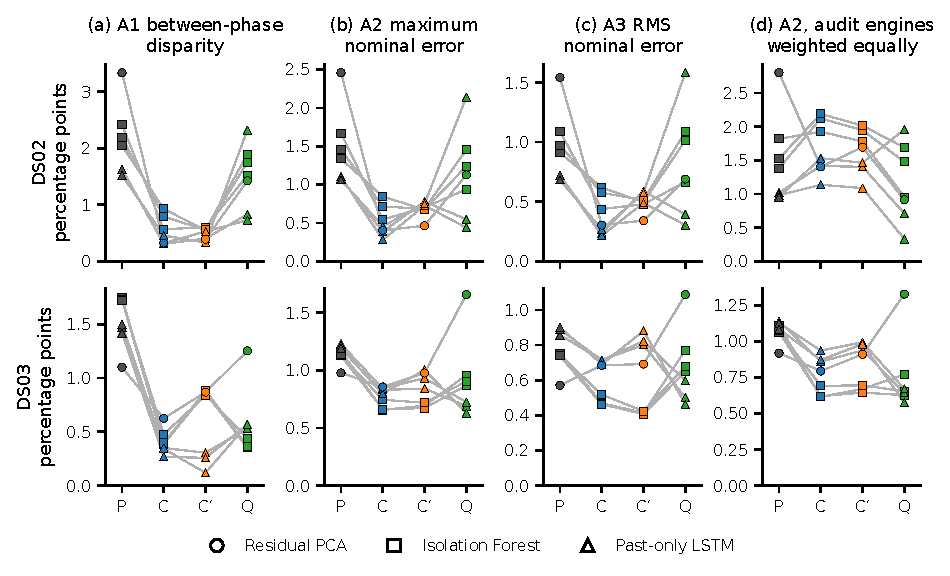
\includegraphics[width=\textwidth]{../figures/fig3_disparity_and_nominal_calibration.pdf}
\caption{Between-phase disparity and nominal calibration error at the 1\% target under pooled (P), retrospective phase-conditioned (C), past-only regime-conditioned (C′) and continuous contextual (Q) calibration; one grey line per detector run. Panels (a–c) are row-pooled over audit engines, and panel (d) weights audit engines equally. All paired arm-minus-P bootstrap intervals include zero.}
\label{fig:3}
\end{figure}
\begin{itemize}
\item DS02: from 1.52–3.33 to 0.31–0.92 pp;
\item DS03: from 1.10–1.75 to 0.27–0.63 pp.
\end{itemize}

Past-only regime-conditioned calibration (C′) also reduced it in every run, to DS02 0.33–0.60 and DS03 0.12–0.88 pp. The continuous baseline Q reduced disparity relative to P in 12 of 14 runs.

\textbf{Uncertainty.} None of the paired arm-minus-P intervals for disparity excluded zero.

\textbf{Engine heterogeneity.} Disparity reduction did not hold in every engine (Section 4.8.5).

\textbf{Interpretation.} Because calibration and audit engines were disjoint, the pooled reduction is out of sample. Most of the pooled phase disparity therefore comes from calibrating one threshold over a mixture of phases.

\subsubsection{Nominal calibration error}

\textbf{Point estimate.} The disparity reduction was not only an equalization of phases around a biased level. For the row-pooled audit population, C also reduced the maximum nominal calibration error A2 in all 14 runs and the RMS error A3 in 13 of 14 runs at 1\% (Fig. 3b,c):
\begin{itemize}
\item DS02: A2 fell from 1.06–2.46 to 0.28–0.85 pp;
\item DS03: A2 fell from 0.98–1.23 to 0.66–0.86 pp.
\end{itemize}

\textbf{Categories.} C fell in category 1 (disparity and nominal calibration both improve):
\begin{itemize}
\item DS02: 7 of 7 runs at every target;
\item DS03: 7, 6, and 5 of 7 runs at 0.5\%, 1\% and 2\%.
\end{itemize}

\textbf{Overall rate.} Overall healthy FPR moved by −0.10 to +0.40 pp, and its error A5 improved in only 4 of 14 runs. Conditioning therefore redistributed healthy alarms across phases rather than reducing them.

\textbf{Uncertainty.} No paired arm-minus-P interval excluded zero at 1\%, for any metric, arm or dataset. At 0.5\% and 2\%, 558 of 560 paired U1 intervals included zero. The two exceptions were disparity reductions by C′ for DS02 Isolation Forest seeds 0 and 1 at 2\%.

\textbf{Interpretation.} Under the pre-specified wording rule, only DS02 C qualifies for ``improved nominal phase-wise calibration'' on the row-pooled estimand. DS03 C and both C′ arms qualify only for ``reduced between-phase disparity''. The 14 of 14 count is a directional pattern, not an inferential result.

\subsubsection{Row-pooled versus equal-engine weighting}

\textbf{Point estimate.} The row-pooled estimand gives most weight to the engines with the most healthy rows. With the audit engines weighted equally, the DS02 improvement reversed (Fig. 3d, Table 5). C fell in category 4, worsening both disparity and nominal calibration, in 5 of 7 runs at 1\%, and its equal-engine A2 was higher than under P in 6 of 7 runs. On DS03, the equal-engine results agreed with the row-pooled ones: category 1 in 6 of 7 runs and no run with a higher equal-engine A2.
\begin{table}[htbp]
\centering
\small
\caption{Detection delay at matched healthy-flight false-flag burden (1\% row target). Anchor columns give earlier/tie/later run counts of the paired lower-median delay difference against P at supported anchors. The table also gives the pre-specified run labels (earlier/mixed/equal/later), the realized pooled false-flag rates at the locked κ, and the curve-level mean delay difference (flights).}
\label{tab:4}
\begin{adjustbox}{max width=\textwidth}
% Detection delay at matched healthy-flight false-flag burden (1% row target)
\begin{tabular}{lllllllllll}
\toprule
Dataset & Arm & 2.5\% & 5\% & 10\% & 15\% & 20\% & \makecell{Run labels\\E/M/=/L} & \makecell{Locked FFR,\\P (\%)} & \makecell{Locked FFR,\\arm (\%)} & \makecell{Curve-mean\\difference (flights)} \\
\midrule
DS02 & C & 5/0/0 & 7/0/0 & 2/1/1 & 2/4/1 & 1/5/0 & 3/4/0/0 & 6.6--19.7 & 9.2--19.7 & $-$4.93 to +0.04 \\
 & C$'$ & 5/0/0 & 6/1/0 & 3/1/1 & 4/0/3 & 1/2/2 & 4/3/0/0 & 6.6--19.7 & 11.8--31.6 & $-$5.41 to +2.54 \\
\midrule
DS03 & C & 4/2/1 & 3/2/1 & 0/6/0 & 0/5/0 & 0/6/0 & 0/5/2/0 & 2.7--16.2 & 2.7--19.6 & $-$2.56 to +3.09 \\
 & C$'$ & 5/2/0 & 3/3/0 & 3/3/1 & 1/3/0 & 1/5/0 & 2/4/1/0 & 2.7--16.2 & 6.8--20.9 & $-$2.60 to +2.98 \\
\bottomrule
\end{tabular}

\end{adjustbox}
\end{table}
\begin{table}[htbp]
\centering
\small
\caption{Cross-engine transport at the 1\% target: per-engine and equal-engine A2 ranges under P, C and Q, the number of runs in which C or Q is worse than P, and the C-against-P category counts. ``Absent'' marks a flight class not represented among that dataset's calibration engines.}
\label{tab:5}
\begin{adjustbox}{max width=\textwidth}
% Cross-engine transport of pooled-level calibration gains (1% target)
\begin{tabular}{lllllllll}
\toprule
Dataset & Engine & \makecell{Flight\\class} & A2, P & A2, C & \makecell{C worse\\than P} & \makecell{C categories\\1/2/3/4} & A2, Q & \makecell{Q worse\\than P} \\
\midrule
DS02 & 11 & 3 & 1.23--1.78 & 0.25--0.38 & 0/7 & 7/0/0/0 & 0.44--4.25 & 4/7 \\
 & 14 & 1 (absent) & 0.99--3.97 & 3.74--6.59 & 7/7 & 0/1/0/6 & 0.54--2.20 & 4/7 \\
 & 15 & 2 (absent) & 0.66--2.67 & 0.14--0.30 & 0/7 & 7/0/0/0 & 0.58--4.18 & 3/7 \\
 & \makecell{all (equal\\weight)} & -- & 0.96--2.81 & 1.14--2.19 & 6/7 & 1/1/0/5 & 0.33--1.96 & 3/7 \\
\midrule
DS03 & 10 & 3 & 1.45--3.08 & 1.52--2.56 & 3/7 & 3/3/1/0 & 3.59--7.57 & 7/7 \\
 & 11 & 3 & 1.17--1.67 & 0.49--0.99 & 0/7 & 7/0/0/0 & 0.56--0.89 & 0/7 \\
 & 12 & 1 (absent) & 0.39--0.85 & 0.82--2.17 & 7/7 & 0/0/0/7 & 0.40--0.74 & 4/7 \\
 & 13 & 3 & 1.25--1.81 & 0.77--1.47 & 0/7 & 6/0/1/0 & 0.58--1.69 & 2/7 \\
 & 14 & 1 (absent) & 0.31--0.74 & 0.37--0.76 & 3/7 & 4/0/0/3 & 0.30--0.97 & 6/7 \\
 & 15 & 2 & 0.38--1.15 & 0.25--1.28 & 4/7 & 3/2/1/1 & 0.49--0.66 & 4/7 \\
 & \makecell{all (equal\\weight)} & -- & 0.92--1.14 & 0.62--0.94 & 0/7 & 6/0/1/0 & 0.58--1.33 & 1/7 \\
\bottomrule
\end{tabular}

\end{adjustbox}
\end{table}

\textbf{Sign agreement.} The signs of the calibration-error changes (A2, A3) agreed between the two weightings in 15–16 of 42 DS02 comparisons and in 36–39 of 42 DS03 comparisons, counted over runs, targets and both conditioned arms.

\textbf{Decomposition.} A post-plan descriptive decomposition treats engine × phase cells equally (Supplementary Table S23 and Fig. S4). Under P, the phase component dominated the mean squared nominal error, with medians of 72\% (DS02) and 57\% (DS03). Under C it fell to 14\% and 5\%. The equal-cell RMS error, however, rose on DS02 (1.61 against 0.96 pp) and was essentially unchanged on DS03 (0.81 against 0.84 pp).

\textbf{Interpretation.} Conditioning converted most of a phase-composition error into engine and engine × phase error. Whether it helps depends on the weighting, and the operationally relevant weighting depends on the deployment.

\subsubsection{Matched false-flag detection delay}

\textbf{Why matching is needed.} Comparisons at the locked κ were potentially confounded, because the locked κ did not transport. Realized pooled healthy-flight false-flag rates ranged from 2.7–31.6\% against a nominal 5\%, and one class-1 engine reached 57\% (Fig. 4c). Delays were therefore compared at matched realized FFR, using supported operating points only.
\begin{figure}[htbp]
\centering
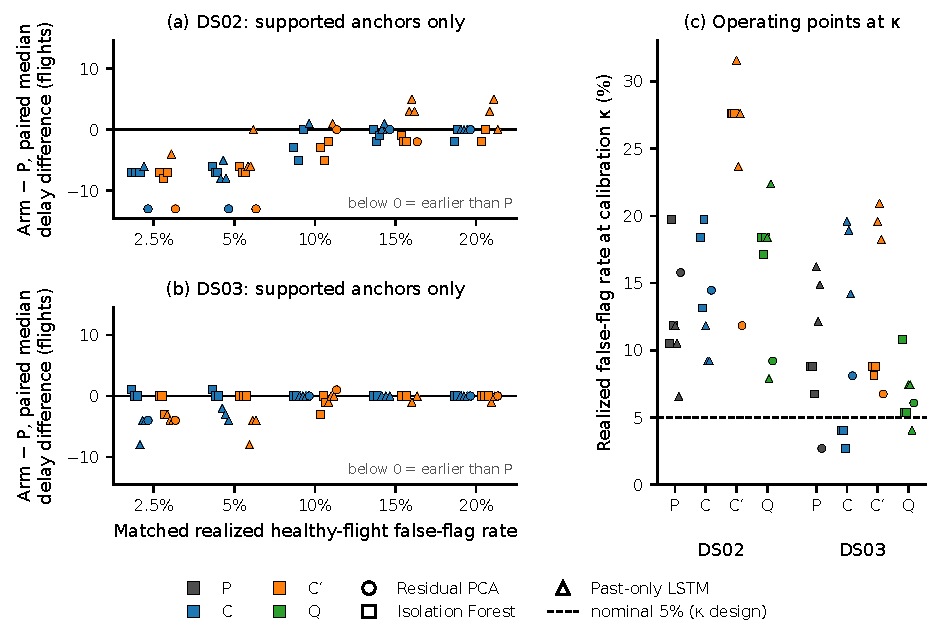
\includegraphics[width=\textwidth]{../figures/fig4_matched_false_flag_tradeoff.pdf}
\caption{Detection delay at matched healthy-flight false-flag burden (1\% row target). (a, b) Paired lower-median per-engine delay difference (arm minus P, flights) at each matched realized false-flag rate, for supported anchors only (within one healthy-flight step), without interpolation; negative values mean earlier detection. Counts are in Table 4. (c) Realized pooled healthy-flight false-flag rate at the calibration-locked κ (P, C, C′) and at Q's calibration κ; the dashed line is the nominal 5\% design rate.}
\label{fig:4}
\end{figure}

\textbf{Matched comparisons, point estimates} (Fig. 4a,b; Table 4):
\begin{itemize}
\item \textbf{DS02, low burden.} C flagged abnormal-state onset earlier than P at the lowest anchors: 5 of 5 supported runs at 2.5\%, and 7 of 7 runs at 5\% (median paired difference −7 flights).
\item \textbf{DS03, low burden.} Earlier in 4 of 7 runs at 2.5\% (one later), and in 3 of 6 supported runs at 5\% (one later).
\item \textbf{Higher burdens.} At 10\% or more, the differences largely vanished (mostly ties), and median delays were at most 7 flights in every arm.
\end{itemize}

\textbf{Pre-specified labels.} Because of these ties, ``earlier at matched burden'' held in only 3 of 7 DS02 runs and 0 of 7 DS03 runs for C, and in 4 and 2 of 7 for C′. The pre-specified criterion for ``improves detection delay'' was therefore not met. The curve-level mean delay over 2.5–20\% FFR was lower for C than for P in 6 of 7 runs on each dataset, but that is only the second condition of the criterion.

\textbf{Uncertainty.} No interval was attached to the matched differences (three and six audit engines); per-engine values are in the Supplement.

\textbf{Locked points.} At the locked κ, most comparisons were trade-offs: one arm had the lower delay and the other the lower false-flag rate. The apparent locked-point delay advantages therefore mainly reflected more aggressive flight-level operating points, especially on DS03.

\textbf{Row-level rates.} Abnormal-state row alarm rates stayed within the interpretive guardrails (family ratios 0.98–1.16). Row-level alarm rates and flight-level delays often moved in different directions, so neither substitutes for the other. The frozen burden endpoint ``healthy flights with any alarm'' and the κ-based FFR also changed in opposite directions in most runs (Supplementary Tables S12 and S17).

\textbf{Interpretation.} Conditioning offered a trade-off concentrated at low false-flag burden: it did not dominate P, and it gave no general delay advantage.

\subsubsection{Cross-engine failures and flight-class composition}

\textbf{Class-1 engines.} Calibration contained no class-1 engine in either subset. Conditioning worsened A2 and A3 in every detector run at 1\% for two of the three class-1 audit engines (Fig. 5, Table 5):
\begin{figure}[htbp]
\centering
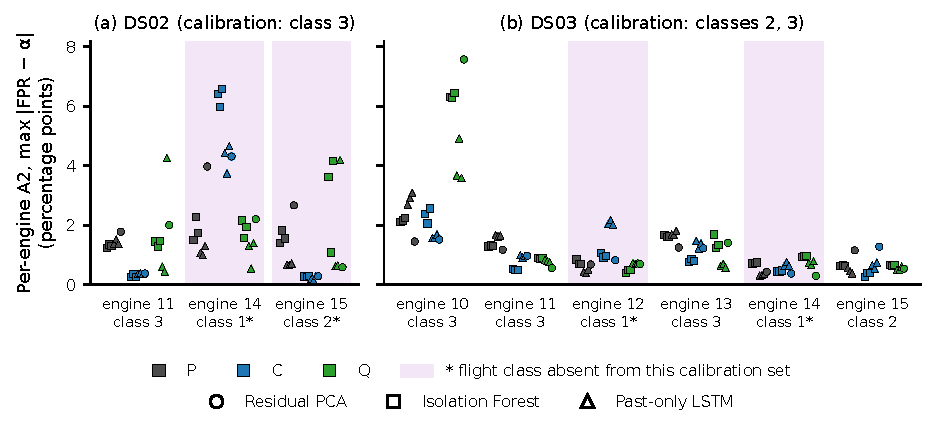
\includegraphics[width=\textwidth]{../figures/fig5_engine_transport.pdf}
\caption{Per-engine transport at the 1\% target: maximum nominal calibration error A2 of each audit engine for every detector run under P, C and Q. Shading and asterisks mark engines whose flight class is absent from that dataset's calibration set: class 1 in both subsets, and class 2 in DS02. DS02 calibration engines are class 3; DS03 calibration engines are classes 2 and 3.}
\label{fig:5}
\end{figure}
\begin{itemize}
\item \textbf{DS02 engine 14.} A2 rose from 0.99–3.97 pp under P to 3.74–6.59 pp under C. Climb, which over-alarmed under C, carried the largest error.
\item \textbf{DS03 engine 12.} A2 rose from 0.39–0.85 to 0.82–2.17 pp.
\item \textbf{DS03 engine 14.} This third class-1 engine worsened in 3 of 7 runs.
\end{itemize}

The past-only regime arm showed the same engine-level pattern: its A2 exceeded that of P for DS02 engine 14 in 7 of 7 runs and for DS03 engine 12 in 6 of 7.

\textbf{Other absent-class and in-class engines.} Not every engine from a class absent from calibration failed. DS02 engine 15 (class 2, also absent from DS02 calibration) improved under C in every run, with A2 falling from 0.66–2.67 to 0.14–0.30 pp. Some in-class engines worsened in several runs: DS03 engine 10 (class 3) in 3 of 7 runs and DS03 engine 15 (class 2) in 4 of 7.

\textbf{Interpretation.} This is descriptive evidence from three class-1 engines and one class-2 engine, without per-engine intervals. The largest and most consistent failures coincided with the class that no calibration engine represented, which points to calibration composition and transport. It does not establish flight class as the causal variable, and flight class was never used to change a rule.

\subsubsection{Continuous contextual baseline}

\textbf{Calibration.} The in-sample calibration alarm rate of Q (Section 3.9.2) was 0.97–1.03\% at the 1\% target.

\textbf{Pooled point estimates} (Fig. 3, Table 3). Q reduced disparity relative to P in 12 of 14 runs. However, its row-pooled maximum phase error was lower than that of C in only 3 of 14 runs (0 of 7 on DS02).

\textbf{Engine heterogeneity} (Fig. 5, Table 5):
\begin{itemize}
\item \textbf{Class-1 engines.} Q transported better than C to the two engines on which C failed. DS02 engine 14 had a maximum phase error of 0.54–2.20 pp under Q against 3.74–6.59 pp under C, and DS03 engine 12 had 0.40–0.74 against 0.82–2.17 pp.
\item \textbf{In-class engines.} Q failed where C did not. DS03 engine 10 (class 3) reached 3.59–7.57 pp, worse than P in every run, and on DS02 single runs reached up to 4.25 pp on engines 11 and 15.
\item \textbf{Flight level.} The realized healthy-flight false-flag rate at Q's calibration κ was 7.9–22.4\% (DS02) and 4.1–10.8\% (DS03).
\end{itemize}

\textbf{Interpretation.} Neither discrete phase conditioning nor the tested continuous contextual calibration produced uniformly transportable calibration across engines. Because the two failed on different engines, the transport failure is not solely an artefact of coarse phase discretization. Q is one transparent baseline, not an exhaustive search over contextual models, and its abnormal-state side was not evaluated.

\subsubsection{Operating-support-distance analysis}

\textbf{The phase effect needs no support mismatch.} Applied to the calibration engines themselves, the pooled threshold reproduced the phase ordering (Fig. 6a). In-sample, descent was the highest-FPR phase in 7 of 7 runs on each dataset:
\begin{figure}[htbp]
\centering
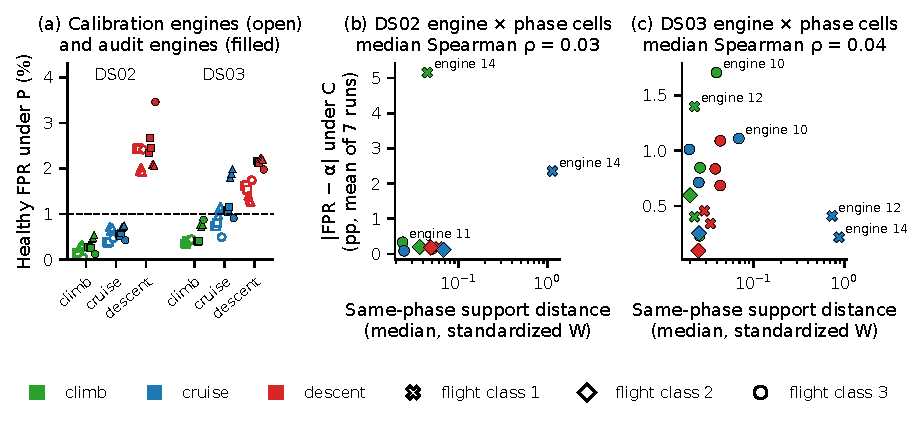
\includegraphics[width=\textwidth]{../figures/fig6_operating_context_and_support.pdf}
\caption{Operating context and support. (a) Pooled-threshold phase FPR within the calibration engines (in-sample; open markers) and in the audit engines (filled), one marker per detector run. (b, c) Median same-phase support distance against |FPR − α| under C for each audit engine × phase cell (mean over the seven runs), with the median per-run Spearman correlation. Descriptive; no p-values are computed.}
\label{fig:6}
\end{figure}
\begin{itemize}
\item DS02: descent 1.92–2.45\% against climb 0.04–0.32\%;
\item DS03: descent 1.27–1.74\% against climb 0.35–0.45\%.
\end{itemize}

Descent was also highest in 27 of 28 run–target combinations at 0.5\% and 2\%, and in 27 of 28 evaluations from one calibration engine to the other at 1\%. The pooled phase effect is therefore a property of the healthy score distribution that a pooled threshold averages over, not a product of calibration-to-audit mismatch.

\textbf{Where the class-1 engines leave support.} Their cruise rows lay far from calibration cruise states (Fig. 6b,c; Supplementary Table S20):
\begin{itemize}
\item a median same-phase distance of 0.74–1.13, against at most 0.07 for every other engine × phase cell;
\item 82–95\% of their cruise rows outside the calibration cruise range.
\end{itemize}

Their climb and descent rows lay within support.

\textbf{Distance did not explain the residual failures.} The largest residual errors under C occurred in cells that were within support: DS02 engine 14 climb and DS03 engine 10 climb (class 3). Across engine × phase cells, the Spearman correlation between support distance and |FPR − α| under C had a median of 0.03 (DS02) and 0.04 (DS03), and its sign flipped when single engines were left out. The pre-specified verdict was \emph{indeterminate due to the small engine count}. Descriptively, nearest-neighbour operating-state distance did not explain the residual transport failures. The largest failures sat on class-1 engines, not on the cells farthest from calibration support.

\section{Discussion}

\subsection{What pooled calibration misses}

As the mixture decomposition implies, a pooled nominal target controls an exposure-weighted average and can conceal large differences in $P(\mathrm{alarm}\mid\mathrm{healthy},\mathrm{phase})$. The effect has four features:
\begin{itemize}
\item it appeared in discovery and reproduced under the frozen confirmation;
\item it was present within the calibration engines themselves, at every target and for three detector implementations;
\item it is therefore a property of the healthy score distribution under the tested corrections, not an artefact of moving thresholds between engines;
\item the tested corrections did not sufficiently attenuate it.
\end{itemize}

That last point is a bounded statement about these fitted corrections. Finite sensor response, omitted operating variables, longer state history, path dependence and simulator structure remain hypotheses. Phase is a retrospective stratum here, not a physical cause.

\subsection{Why lower phase disparity is not sufficient}

A threshold rule can equalize phases around the wrong level, or equalize them for the pooled population while individual engines diverge. The post-confirmation results show the second failure:
\begin{itemize}
\item Pooled disparity and pooled nominal error fell.
\item Overall healthy FPR was not reduced; alarms were redistributed across phases.
\item With engines weighted equally, the DS02 improvement reversed, because most of the pooled phase-composition error became engine and engine × phase error.
\end{itemize}

A context-specific calibration rule can therefore look successful when evaluated after pooling across engines, yet fail on engines outside the calibration composition. Reporting disparity alone, or only the row-pooled estimand, would have hidden this.

\subsection{Calibration transport across engines}

Calibration guarantees are statements about exchangeable data \cite{N20}. Marginal validity is an average over calibration sets, a particular calibration set can be unrepresentative \cite{N16}, and transfer under covariate shift requires reweighting \cite{N30}. Monitoring models likewise transfer poorly beyond the systems and conditions they were built on \cite{N21}, and fleet-level normal models can be inefficient at heterogeneous individual units \cite{N44}. On N-CMAPSS, flight phases differ between flight classes \cite{N28}, and the class-1 cruise rows lie outside the calibration cruise support.

Three observations nevertheless bound any composition explanation:
\begin{enumerate}
\item \textbf{Support distance.} Class-1 climb rows were within support yet over-alarmed under C.
\item \textbf{An absent-class engine that improved.} DS02 engine 15 came from a class absent from calibration, yet it improved in every run, so class absence was not sufficient for failure.
\item \textbf{The continuous baseline.} Q moved the failure to other engines.
\end{enumerate}

Together they suggest an engine- or flight-profile-level shift in the healthy score distribution conditional on operating state, which neither phase labels nor the tested operating descriptors captured. That is a hypothesis for future work. The strongest observed transport failures coincided with the flight class absent from calibration, but three engines cannot establish flight class as the governing variable.

\subsection{Implications for machine-health-monitoring evaluation}

Context-specific false-alarm calibration should not be judged only by aggregate or phase-pooled improvements. Its transport should be audited across engines and operating classes, with nominal calibration error, between-context disparity and detection/false-flag trade-offs reported jointly. Concretely, a monitoring evaluation should report:
\begin{itemize}
\item phase- or context-conditional healthy FPR alongside the pooled FPR;
\item nominal calibration error, not only between-context disparity;
\item row-pooled and equal-engine summaries, with every engine exception;
\item the composition of the calibration set (engines, flight classes and operating ranges) relative to the units on which thresholds are used;
\item detection delay as an operating characteristic against realized false-flag burden, compared at matched burden and without interpolation.
\end{itemize}

These are evaluation requirements, not evidence that any threshold policy is superior. Phase-conditioned thresholds are not recommended here as a deployment solution.

The staged design mattered: freezing and a one-shot confirmation separated exploration from the confirmatory claim \cite{N33}, and the frozen post-confirmation plans exposed the weighting dependence, the transport failure and the matched-burden delay pattern, all of which would have been easy to explain away afterwards.

\subsection{Relation to prior context-aware methods}

This study does not compete with context-aware monitoring methods; it evaluates the calibration question that they raise:
\begin{itemize}
\item \textbf{Mode- and condition-specific thresholds.} Mode-specific control limits \cite{N8}, per-condition extreme-value alarms \cite{N22}, speed-binned engine thresholds \cite{N27}, flight-condition segmentation \cite{N25} and flight-state thresholds \cite{N26} all motivate context-specific thresholds by false alarms. Our results support that motivation for the pooled population: C removed most of the phase-composition error. They add that such an improvement need not transport to engines outside the calibration composition.
\item \textbf{Per-mode false-positive rates.} Michau and Fink showed that a single-mode calibration fails in other modes \cite{N23}. Here, even with every phase present in calibration, a per-phase calibration failed on two of the three engines of an unrepresented flight class.
\item \textbf{Delay at a fixed false-alarm budget.} ProDiMES compared detection latency at a fixed flight-level false-alarm target \cite{N24}, and sequential detection defines delay at a fixed false-alarm rate \cite{N17}. Our matched analysis applies the same principle to calibration arms and shows how locked-point comparisons can mislead when the flight-level threshold does not transport.
\item \textbf{Alarm-system design.} Joint false-alarm, missed-alarm and delay design \cite{N32}, including time-variant and zone-specific designs for non-stationary process variables \cite{N39,N40}, shares our insistence on evaluating false alarms and delay together. Here the contexts are normal flight phases rather than fault-evolution stages, and the question is whether a context-specific calibration transports across units. The same question applies to the thresholds of context-conditioned detectors \cite{N38} and of conformally calibrated detectors \cite{N41}.
\end{itemize}

\subsection{Limitations}
\begin{itemize}
\item \textbf{Simulated data.} N-CMAPSS is a simulation driven by recorded flight conditions. The results do not establish validity on real aircraft, and there was no real-aircraft validation.
\item \textbf{Few engines.} There are only two calibration engines per dataset and three (DS02) and six (DS03) audit engines. Class-1 transport evidence rests on three engines in total, and absent-class evidence on four.
\item \textbf{Intervals.} All primary paired post-confirmation intervals include zero. Every post-confirmation statement is a point-estimate pattern, and the support association is indeterminate.
\item \textbf{Post-confirmation status.} The post-confirmation analyses were frozen before execution but are exploratory. They reuse the confirmation engines and are not part of the DS03 confirmation.
\item \textbf{Retrospective phases.} Phase labels require complete trajectories. The retrospective phase-conditioned arm is a diagnostic, not an implementable monitor.
\item \textbf{Simulated labels.} The abnormal-state label ($hs = 0$) is a simulated degradation-state annotation, not a discrete real-aircraft fault event, and delays are measured from that labelled onset.
\item \textbf{Baseline scope.} The continuous contextual baseline is one transparent specification, not an exhaustive search. Its abnormal-state side was not evaluated.
\item \textbf{No mechanism.} The operating-support metrics tested do not identify a mechanism. The flight-class association is descriptive, not causal evidence.
\item \textbf{Shared pipeline.} The detector families share preprocessing, residualization and calibration, so they are not independent replications. Seed means are descriptive.
\item \textbf{Implementation.} No independent implementation or reimplementation of the pipeline exists. The analysis code was developed with AI assistance and verified by the author (see the declaration below).
\end{itemize}

\section{Conclusion}

\textbf{What was discovered and confirmed.} Pooled healthy calibration of full-flight aero-engine anomaly detectors left false-alarm rates dependent on flight phase. The dependence was discovered on DS02, the pre-specified pooled directional pattern reproduced under a frozen one-shot DS03 protocol, and the same ordering was present within the calibration engines.

\textbf{What the transport audit changed.} Post-confirmation, retrospective phase-conditioned thresholds reduced pooled between-phase disparity and pooled nominal calibration error in every detector run, although all paired intervals included zero. The correction did not transport reliably to individual engines. The strongest failures coincided with the flight class absent from calibration, equal-engine weighting reversed the DS02 improvement, a continuous contextual threshold failed on other engines, and operating-support distance did not explain the failures. At matched false-flag rates, conditioning gave no general detection-delay advantage.

\textbf{Why pooled correction is insufficient.} A context-specific calibration rule can look successful when evaluated after pooling across engines yet fail on engines outside the calibration composition. Full-flight anomaly-detection studies should therefore evaluate not only conditional false-alarm disparity but also calibration transport across engines and operating classes.

\textbf{What remains to be validated.} The evidence is limited to simulated N-CMAPSS subsets and small engine sets, and it identifies no mechanism. Future validation should use real or independently sourced full-flight data, calibration sets that deliberately span the flight classes and operating ranges to which thresholds will be applied, and frozen transport tests on units held out from calibration.

\section*{Data availability}

N-CMAPSS is publicly available from the NASA Prognostics Center of Excellence Data Set Repository (``Turbofan Engine Degradation Simulation-2''). This study used subsets DS02 and DS03. The raw NASA files are not redistributed.

\section*{Code availability}

Code, frozen protocols and plans, run records, derived outputs and the scripts that re-derive every reported number are available at https://github.com/surnamemei/ncmapss-phase-entanglement. The MSSP version corresponds to release v1.1.0, which is to be archived with a persistent identifier before publication.

\section*{Declaration of competing interest}

The author declares no known competing financial interests or personal relationships that could have appeared to influence the work reported in this paper.

\section*{Funding}

This research did not receive any specific grant from funding agencies in the public, commercial, or not-for-profit sectors.

\section*{CRediT authorship contribution statement}

\textbf{Jinghang Mei:} Conceptualization, Methodology, Software, Validation, Formal analysis, Investigation, Data curation, Visualization, Writing – original draft, Writing – review \& editing.

\section*{Appendix A. Supplementary data}

The supplementary material (Tables S1–S23 and Figures S1–S4) and machine-readable evidence files accompany this article.

\section*{Declaration of generative AI and AI-assisted technologies in the manuscript preparation process}

During the preparation of this work, the author used OpenAI ChatGPT and Codex (OpenAI) and Claude (Anthropic; Claude Opus 5.5, through the Claude Code tool) in order to assist with code development and debugging (described in Section 3.10), literature searching, organization of the literature and verification of references, and drafting and editing of substantial parts of the manuscript text, figure captions, tables and supplementary material. After using these tools, the author reviewed and edited the content as needed and takes full responsibility for the content of the published article.


\bibliographystyle{elsarticle-num}
\bibliography{references_mssp}
\end{document}
